\chapter{Results}
%In this chapter, you should discuss the results you have obtained from your implementation.
%These can be correctness results, i.e whether the implementation behaved as expected, or numerical results that express runtime or energy measurements.
At first there were some issues with the arithmetics in both the Blakley and Monpro modules due to integer overflow. Some times the result would be aligned incorrectly, other times it would be all zero, and on rare occasions the compiler would crash with no error messages.\\

After implementing and testing the design (and submodules), we discovered that the output matched the expected results from the python implementation, but not the expected results from the provided system testbench. This means that the python model was probably wrong, or the provided test data is.

\section{Synthesis and test on FPGA}
\subsection{Synthesis results (Vivado)}
The results shown in figure \ref{fig:utilization} and table \ref{tab:vivado_synth_results} are obtained from Xilinx Vivado after running the synthesis and implementation steps, using RSACore as the top level of the design hierarchy.
\begin{figure}[H]
\centering
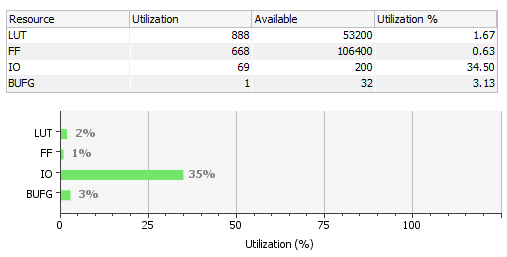
\includegraphics[width=\textwidth]{images/Vivado_utilization}
\caption{Utilization report from Vivado}
\label{fig:utilization}
\end{figure}

TODO: figure with Vivado\_timing.PNG here

\begin{table}[H]
    \centering
    \begin{tabular}{l|r}
        Metric & Value \\ \hline
        Power (total) & 0.133W\\
        Power (dynamic) & 0.013W \\
        Power (static) & 0.120W \\
    \end{tabular}
    \caption{Vivado power consumption}
    \label{tab:vivado_synth_results}
\end{table}
\subsection{Measure area and performance}
As the design did not pass the functionality tests there are no actual performance results available. However it is reasonable to assume that the Blakley algorithm will take 128 clock cycles to complete and the Monpro will take 129, seeing as there was not enough time to start optimizing the iterations by stopping earlier.\\
Therefore a rough estimate is between $4+128+(128*129)+4$ ($key_e$ of all 0's) and $4+128+2*(128*129)+4$ cycles ($key_e$ of all 1's), with the average probably close to the lower of the two because a small $key_e$ is common to use (TODO: citation).


\section{Discussion of the results}
 
Analysis and discussion of problems, solutions and measured results is necessary in order to make the right decisions. Discussion should therefore be integrated into all parts of the report. 

The complexity of the Montgomery algorithm vs if we had implemented a blakley for the modular multiplications. 
- What is done, what can be improved (future work).

\section{Further improvements}
In order to improve performance of the circuit, multiple tricks can be used. Probably most significant is the option to prematurely stop computing when more iterations will not make any difference.\\
For Monpro (see algorithm below), this means to stop once all the bits to the left of the current one are zero; then there will be no more additions

\inputminted[fistline=13,lastline=26]{python}{../Project/monexp.py}
